\vspace*{1.5pc}


%%%%%%%%%%%%%%%%%%%%%%%%%%
\subsection{Initial Conditions}
%%%%%%%%%%%%%%%%%%%%%%%%%%

Generating the initial conditions for our whole set of particles $\left( \vec{r}, \vec{v} \right)$ at a specific time $t$ (here encoded in the cosmological redshift $z \propto a^{-1}$) is no trivial task as errors can potentially be amplified by the simulation. 


\subsubsection{Pre-initial Conditions}
\label{sec:glass}

In this sub-section, I go through the set of \emph{pre}-initial conditions for our N-body + SPH code, \textit{i.e.} the distribution of $\pmb{\Xi}(t_{\mathrm{ic}}) \doteq \left( \vec{r}(t_{\mathrm{ic}}), \vec{v}(t_{\mathrm{ic}}) \right)^T$ representing an unperturbed system. A pioneering study of pre-initial conditions can be found in \citet{White1994} and a more recent one in \citet{LHuillier2014}. A legitimate distribution is the so-called \emph{glass} configuration. It is a compromise between a grid distribution and a uniform distribution (see Fig.~\ref{fig:preinitial_conditions}). \\


Randomly placing particles following a uniform law strongly suffers from Poisson noise and its initial power spectrum corresponds to that of white noise. Evolving such a distribution would lead to the formation of non-linear structures, which should not be the case if no perturbations have been set yet. Placing the particles on a regular grid implies preferred directions along the axis that may develop into artefacts, especially at small scale. Currently, the preferred solution is the aforementioned glass distribution \citep{White1994}. It is constructed by inverting the gravitational evolution (as if the force was repulsive) on a randomly seeded Poisson distribution, and removing large-scale power as in the random distribution and suppressing preferred direction as in the grid distribution. 
	
\begin{figure}
\centering
\begin{subfigure}{0.32\textwidth}
\centering
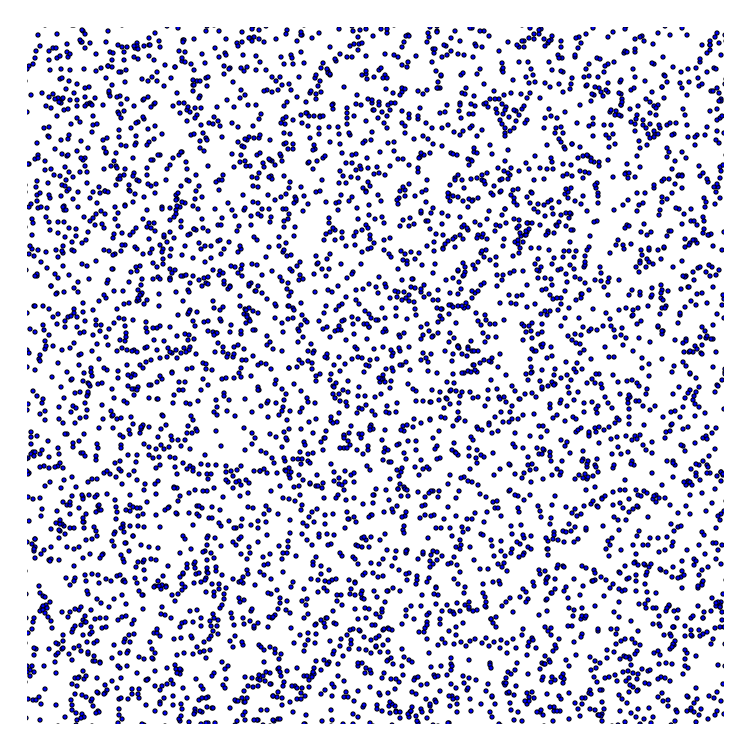
\includegraphics[width=\textwidth]{Simu/uniform.png}
\caption{Random uniform distribution}
\end{subfigure}
\hfill
\begin{subfigure}{0.32\textwidth}
\centering
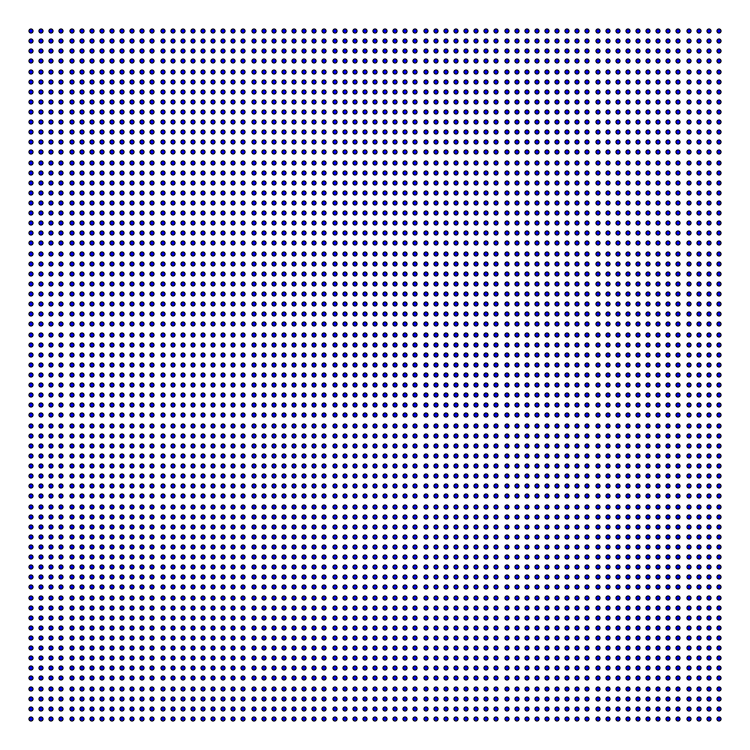
\includegraphics[width=\textwidth]{Simu/grid.png}
\caption{Grid distribution}
\end{subfigure}
\hfill
\begin{subfigure}{0.32\textwidth}
\centering
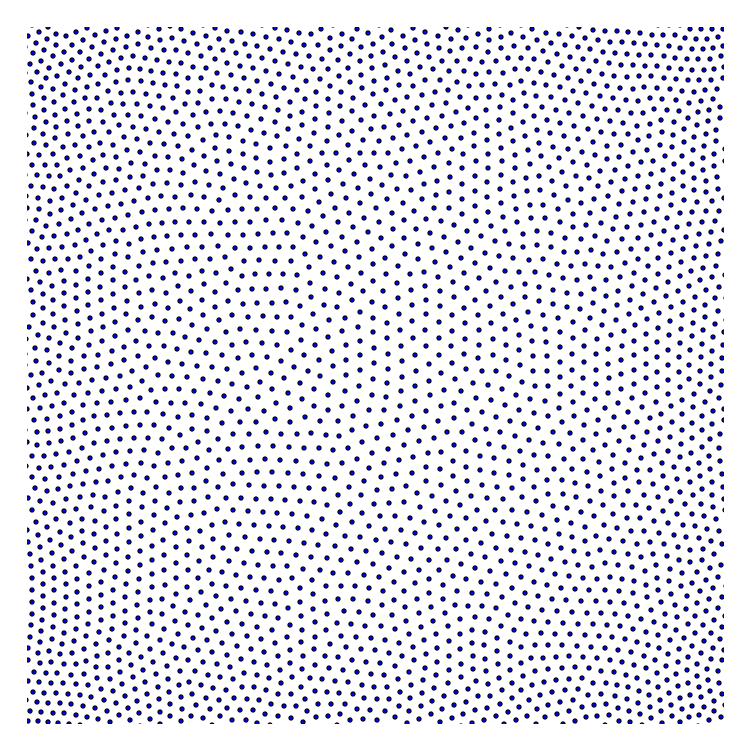
\includegraphics[width=\textwidth]{Simu/glass.png}
\caption{Glass distribution}
\end{subfigure}
\caption[Types of pre-initial particles distribution]{Three different types of pre-inital particle distribution: randomly (uniform) placed
particles, particles placed on a regular grid and glass distribution.}\label{fig:preinitial_conditions}
\end{figure}


\subsubsection{Initial Power Spectrum}
\label{sec:ips}

The original quantum density fluctuations that seeded the inhomogeneities and isotropies can be reproduced by a random Gaussian field in a homogeneous and isotropic space. It is a (discretized) field $\phi(\vec{r})$ with a Gaussian $N$-point distribution function. Noting $\vec{x} = \left( x_1, \hdots, x_n \right)$, the probability to have $x_1 = \phi(\vec{r}_1)$, $\hdots$, $x_n = \phi(\vec{r}_n)$ is given by

\begin{equation}
P(\vec{x}) ~d\vec{x} = \frac{d\vec{x}}{2\pi \sqrt{\det C}} ~\exp \left( - \frac{\vec{x} C^{-1} \vec{x}^T}{2} \right)
\end{equation}


where $C$ is the covariance matrix whose components are $C_{ij} = \xi(x_i, x_j)$, the 2-point correlation function. $C$ is given by

\begin{equation}
C ~=~ 
\left(
\begin{matrix}
\sigma^2 & \xi(x_1, x_2) & \hdots & \xi(x_1, x_n) \\
\xi(x_2, x_1) & \sigma^2 & & \xi(x_2, x_n) \\
\vdots & & \ddots & \vdots \\
\xi(x_n, x_1) & \xi(x_n, x_2) & \hdots & \sigma^2
\end{matrix}
\right)
\end{equation} 

Equivalently, in the Fourier conjugate space, the field can be written as a complex number $\tilde{\phi}(\vec{k})$. One can thus uniquely decompose it into an amplitude $\left\vert \tilde{\phi}(k) \right\vert$ and a phase $\varphi$
\begin{equation}
\label{eq:veckphi}
\tilde{\phi}(\vec{k}) = \left\vert \tilde{\phi}(k) \right\vert~e^{i \varphi}
\end{equation}

where $\varphi$ is uniformly distributed. For each value of $k$, the amplitude obeys a Rayleigh probability
distribution function:
\begin{equation}
P(y)~dy = \frac{y ~dy}{\Delta_\phi^2(k)} \exp \left( - \frac{y^2}{2\Delta_\phi^2(k)} \right)
\end{equation} where the field's dimensionless power spectrum $\Delta_\phi^2 = P_\phi (k) \times k^3/2\pi = \sigma_k^2$ is essentially the variance per log $k$ (see Eq.~\ref{eq:variance_ps}). Consequently, the power spectrum of a Gaussian random field is sufficient to describe it. \\

The initial power spectrum just after inflation is given by the Harrison-Zel'dovich expression in Eq.~\ref{def:Harrison}. Here, 

\begin{equation}
P(k) = \mathcal{A}_s \left(\frac{k}{k_\star} \right)^{n_s}
\end{equation} \\ where $k_\star = 0.05~\mathrm{Mpc}$ is the pivot mode, $\mathcal{A}_s \doteq P(k=k_\star)$ and $n_s = \left. d\ln P(k)/d\ln k \right\vert_{k_\star}$ are respectively the (scalar) amplitude and spectral index of the primordial power spectrum. Because it would be to expensive to evolve a system starting at the epoch of inflation, initial conditions are generated at a much lower redshift $z\sim10-100$ with the assumption that the evolution up to the starting point is linear. Therefore, the initial power spectrum of each species (dark matter, radiation, baryons, neutrinos) has to be corrected by a transfer function $T_i$:

\begin{equation}
P_i(k,z) = \mathcal{A}_s \left(\frac{k}{k_\star} \right)^{n_s} ~\left\vert T_i(k,z) \right\vert^2
\end{equation}
computed by numerical codes like \texttt{CMBFAST} \citep{Seljak1996}, its successor
\texttt{CAMB} \citep{Lewis2000}, or \texttt{CLASS} \citep{CLASS}. The transfer function of the neutrino and dark matter intrinsically depend on their phase-space distribution function. For the RPSN models --- assuming dark matter is resonantly-produced sterile neutrinos --- the distribution function is evolved with a Boltzmann solver, the results being provided in Sec.~\ref{sec:rpsn_intro}. For the warm dark matter models with thermal relics or non-resonantly produced sterile neutrinos, and mixed C+WDM, the distribution function is assumed to be a rescaled Fermi distribution (Eq.~\ref{eq:fs}). For the C+HDM model --- benchmark CDM with massive active neutrinos --- the rescaling factor is simply $1$ since left-handed neutrinos are thermalized. The linear power spectrum is computed using the \texttt{CLASS} code, which also produces the transfer functions for each species. Tab.~\ref{tab:class_param} details the chosen value of input parameters to the software. \\

For the C+HDM and pure WDM simulations, I use the \texttt{CAMB} software instead, since the distribution function of thermalized neutrinos and thermal relics is quasi indistinguishable from a Fermi Dirac distribution, which is internally modeled in the code. When using \texttt{CAMB}, the only free parameter that sets the distribution function --- besides the cosmological parameters $\Omega_{\mathrm{dm}}$, $m_\nu^{\mathrm{eff}}$, $h$, \textit{etc.} --- is the departure from the effective number of thermalized neutrino species $\Delta N_{\mathrm{eff}}$. This is done using the \texttt{nu\_mass\_degeneracies} input parameter in the 2014 version of the code and onwards, assuming the \texttt{share\_delta\_neff} boolean variable is set to false. Tab.~\ref{tab:camb_param} details how each relevant input parameter is set. \\

\begin{table}
	\begin{center}
	\begin{small}
		\begin{tabular}{lcccc}
			\textbf{input parameter} &  \multicolumn{3}{c}{\textbf{C+HDM}} & \textbf{C+WDM}\\[2pt]
			\hline \\[-10pt]
			\\[-10pt]
			\texttt{omega\_cdm} & \multicolumn{3}{c}{$1 - \left( \Omega_\Lambda + \Omega_b + \cfrac{\Sigma m_\nu}{93.14~h^2\mathrm{eV}} \right)$} & $\left[ 1 - (\Omega_\Lambda + \Omega_b) \right] ~ \times (1-F_{\mathrm{wdm}})$ \\[2pt]
			\texttt{omega\_neutrino} & \multicolumn{3}{c}{$\cfrac{\Sigma m_\nu}{93.14~h^2\mathrm{eV}}$} & $\left[ 1 - (\Omega_\Lambda + \Omega_b) \right] ~ \times F_{\mathrm{wdm}}$ \\[2pt]
			\\[-10pt]
			 & \textbf{solo} & \textbf{degenerate} & \textbf{ordered} & \\[2pt]
			\texttt{massless\_neutrinos} & $2.046$ & $0.0$ & $0.0$ & $3.046$ \\[2pt]
			\texttt{nu\_mass\_eigenstates} & $1$ & $3$ & $3$ & $1$ \\[2pt]
			\texttt{massive\_neutrinos} & $1$ & $1~~1~~1$ & $1~~1~~1$ & $1$ \\[2pt]
			\texttt{share\_delta\_neff} & \texttt{True} & \texttt{True} & \texttt{False} & \texttt{False} \\[2pt]
			\texttt{nu\_mass\_fractions} & $1$ & $1/3~~1/3~~1/3$ & $\cfrac{m_1}{\Sigma m_\nu}~~\cfrac{m_2}{\Sigma m_\nu}~~\cfrac{m_3}{\Sigma m_\nu}$ & $1$ \\[2pt]
			\texttt{nu\_mass\_degeneracies} & $1.0$ & $1.015~~1.015~~1.015$ & $1.015~~1.015~~1.015$ & $\Delta N_{\mathrm{eff}}$ \\[2pt]						
			\hline \\[-10pt]
		\end{tabular}
	\end{small}
	\end{center}
	\caption{Input values of the \texttt{CAMB} software to implement the two main catagories of non-cold dark matter cosmologies. The first, second and third columns correspond to the benchmark $\Lambda$CDM with massive active neutrinos, assuming a `solo', `degenerate' and `ordered' configurations (see Sec.~\ref{sec:mass_ordering}). The right-most column assumes a sterile neutrino ('solo' configuration alone) as the warm component of dark matter. Note the value of $\Delta N_{\mathrm{eff}}$ differs if the warm component is a thermal relic (see Eq.~\ref{eq:neff_whether}).}
	\label{tab:camb_param}
\end{table}

All simulations are tuned to obtained a given $\sigma_8$ at $z=0$. This is done with a \texttt{python} script\footnote{refered to the \texttt{spnorm} script in the pipeline exhibited in Fig.~\ref{fig:pipeline}} that
rescales the total matter power spectrum $P(k, z_i)$ issued from \texttt{CAMB} or \texttt{CLASS} before generating the initial conditions
such that 
\begin{equation}
\label{eq:sig8norm}
P(k, z=30) = P^{\mathrm{comp}}(k, z=30) \times \left[ \frac{\sigma_8(z=30)}{\sigma_8^{\mathrm{comp}}(z=30)} \right]^2 
\end{equation} where $\sigma_8^{\mathrm{comp}}$ is the value of $\sigma_8$ computed with the \texttt{CAMB} or \texttt{CLASS} code for a chosen cosmological model, and 
\begin{equation}
\sigma_8(z=30) \times \sigma_8^{\mathrm{comp}} (z=0) = \sigma_8 (z=0) \times \sigma_8^{\mathrm{comp}}(z=30)
\end{equation}
This renormalization of the linear power spectrum enables us to avoid rerunning the code with the corresponding initial spectral amplitude $\mathcal{A}_s$. \\

\begin{table}
	\begin{center}
	\begin{small}
		\begin{tabular}{lcccc}
			\textbf{input parameter} &  \multicolumn{3}{c}{\textbf{C+HDM}} & \textbf{C+WDM}\\[2pt]
			\hline \\[-10pt]
			\\[-10pt]
			 \texttt{Omega\_cdm} & \multicolumn{3}{c}{$1 - \left( \Omega_\Lambda + \Omega_b + \cfrac{\Sigma m_\nu}{93.14~h^2\mathrm{eV}} \right)$} & $\left[ 1 - (\Omega_\Lambda + \Omega_b) \right] ~ \times (1-F_{\mathrm{wdm}})$ \\[2pt]
			& \textbf{solo} & \textbf{degenerate} & \textbf{ordered} & \\[2pt]
			\texttt{N\_eff} & $2.046$ & $0.0$ & $0.0$ & $3.046$ \\[2pt]
			\texttt{N\_ncdm} & $1$ & $3$ & $3$ & $1$ \\[2pt]
			\texttt{m\_ncdm} & $\Sigma m_\nu / \mathrm{eV}$ & $\cfrac{\Sigma m_\nu}{3~\mathrm{eV}}~~\cfrac{\Sigma m_\nu}{3~\mathrm{eV}}~~\cfrac{\Sigma m_\nu}{3~\mathrm{eV}}$ & $\cfrac{m_1}{\mathrm{eV}}~~\cfrac{m_2}{\mathrm{eV}}~~\cfrac{m_3}{\mathrm{eV}}$ & $m_{\nu_s} / \mathrm{eV}$ \\[2pt]
			\texttt{Omega\_ncdm} & $\Omega_\nu \doteq \cfrac{\Sigma m_\nu}{93.14~h^2\mathrm{eV}}$ & $\cfrac{\Omega_\nu}{3}~~\cfrac{\Omega_\nu}{3}~~\cfrac{\Omega_\nu}{3}$ & $\cfrac{\Omega_{\nu 1}}{3}~~\cfrac{\Omega_{\nu 2}}{3}~~\cfrac{\Omega_{\nu 3}}{3}$ & $\left[ 1 - (\Omega_\Lambda + \Omega_b) \right] ~ \times F_{\mathrm{wdm}}$ \\[2pt]
			\texttt{T\_ncdm} & $\cfrac{T_\nu}{T_\gamma}$ & $\cfrac{T_\nu}{T_\gamma}~~\cfrac{T_\nu}{T_\gamma}~~\cfrac{T_\nu}{T_\gamma}$ & $\cfrac{T_\nu}{T_\gamma}~~\cfrac{T_\nu}{T_\gamma}~~\cfrac{T_\nu}{T_\gamma}$ & $\cfrac{T}{T_\gamma}$ \\[2pt]				
			\hline \\[-10pt]
		\end{tabular}
	\end{small}
	\end{center}
	\caption{Input values of the \texttt{CLASS} software similar to Tab.~\ref{tab:camb_param}. The quantity $\Omega_{\nu j}$ refers to the quantity $m_j / 93.14~h^2\mathrm{eV}$, with $j=1,2,3$. Note that the non-cold dark matter particle temperature at the bottom right-most cell differs whether it is a thermal relic ($T = T_x$) or a sterile neutrino ($T = T_\nu$).}
	\label{tab:class_param}
\end{table}

The \texttt{Gadget-3} code does not feature a radiation component. Therefore the massive particle approximation for the neutrino component must be valid when non-linearly solving the cosmological perturbations. In all the pure WDM and C+WDM models I investigate, the effective neutrino mass $m_\nu^{\mathrm{eff}} = m_{\nu_s}$ is heavy enough to neglect the thermal velocities of the warm particle at $z=30$ with respect to the box size, and so the signature of these particles is entirely encoded in the density transfer function. For the C+HDM models, the massive active neutrinos have too light enough masses to neglect their thermal velocities at $z=30$. This is where the \texttt{2LPTic} code comes in. \\




\subsubsection{Initiating Positions and Velocities}

To generate an initial overdensity field $\delta(\vec{r})$ in a cubic volume of side length $L$, the standard procedure is the following:\\
\begin{itemize}
\item[$1 /$] Generate the amplitude of $\tilde{\delta}(\vec{k}) = \mathcal{F} \left[ \delta(\vec{r}) \right]$ in each mode $k \in 2 \pi / L ~\mathbb{Z}^{+}$ available in the box by drawing a random variable $\varsigma \in \left] 0, 1 \right]$ from a uniform distribution and setting 
\begin{equation}
\left\vert \tilde{\delta} (k) \right\vert = \sigma_k \sqrt{-2 \ln \varsigma_k}
\end{equation}\\
\\
\item[$2 /$] Generate the phase $\varphi$ by drawing from a random distribution; \\
\\
\item[$3 /$] Compute the inverse Fourier transform of $\left\vert \tilde{\delta} (k) \right\vert~e^{i \varphi}$ to recover the overdensity in real-space; \\
\\
\item[$4 /$] Apply the overdensity field computed in the previous steps to the unperturbed glass distribution $\langle \rho \rangle$ described in Sec.~\ref{sec:glass} to obtain the density field $\rho(\vec{x}) = \langle \rho \rangle (\vec{x}) \left( 1 + \delta (\vec{x}) \right)$. \\
\end{itemize}

The initial particle distribution in position and velocity $\pmb{\Xi}_i(z_{\mathrm{ic}})$ is then retrieved using the Zel'dovich approximation \citep{Zeldovich1970, Shandarin1989}. For each particle $i \in [\![ 1, n ]\!]$,
\begin{equation}
\pmb{\Xi}_i(t) = \left( 
\begin{array}{c}
\vec{r}_i (t) \\
\vec{v}_i (t)
\end{array}
\right) = \left( 
\begin{array}{c}
\vec{x}_i - \mathcal{D}(t) \\
- \cfrac{d \mathcal{D}}{dt} (t) 
\end{array}
\right) ~\nabla \phi (\vec{x}_i)
\end{equation} where $\vec{r}_i$ is the new position of particle $i$ initially sitting at $\vec{x}_i$ (as determined by the pre-initial distribution), $\vec{v}_i$ its peculiar velocity, $\mathcal{D}(t)$ is the growth rate of linear density fluctuations and $\phi$ is the gravitational potential generated by the density field. The expression of $\mathcal{D}(t)$ depends on the chosen cosmology. The Zel'dovich approximation corresponds to the first order of the Lagrangian perturbation theory. A code that generates $\pmb{\Xi}(z_{\mathrm{ic}})$ in this approximation is \texttt{N-GENic} developped by Volker Springer and directly compatible with \texttt{Gadget}. For computational memory purposes, I use this code when running simulations with a very large particle count, \textit{i.e.} $N=1024, 1600, 2048$ where $N^3$ is the number of particles for each species. For more accurate initial conditions, especially for low starting redshifts, the approximation can be pushed to second order \citep{Scoccimarro1998, Crocce2006, LHuillier2014}. This is done with the \texttt{2LPTic}\footnote{\url{http://cosmo.nyu.edu/roman/2LPT/}} code. I run all simulations with $N=192, 768$ with this code. The choice of second order precision initial conditions is motivated by the discussion in \citet{Crocce2006} and including neutrinos as a new particle type~\citep{Rossi2014}. The choice of a rather low redshift $z_{\mathrm{ic}}=30$ (instead of $z_{\mathrm{ic}}=100$ typically) to start the non-linear solving is to reduce Poisson noise \citep{Ali-Haimoud2012a, Bird2011a}. \\



%%%%%%%%%%%%%%%%%%%%%%%%%%%%%%
\subsection{Sampling Variance}
%%%%%%%%%%%%%%%%%%%%%%%%%%%%%%

\begin{figure}
\begin{center}
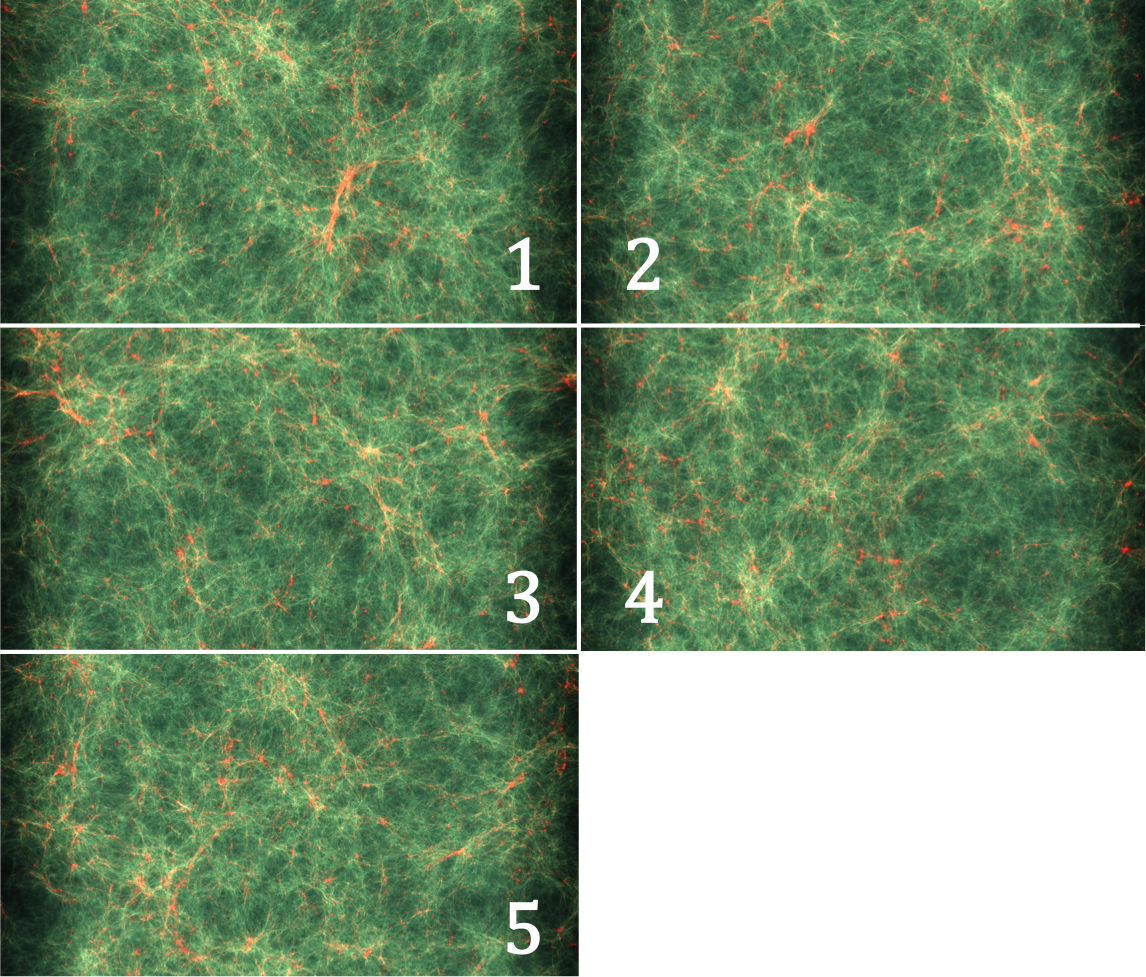
\includegraphics[width=\columnwidth]{Visu/5seeds.png}
\caption{Visual inspection of the $768^3$ baryon gas temperature and density, encoded by color and intensity respectively, in a comoving volume of $100~(h^{-1}\mathrm{Mpc})^3$ using the \texttt{Splotch} software. Each panel corresponds to a different seed $\pmb{\Xi_j}$, $j \in [\![ 1, 5 ]\!]$ when generating the initial position and velocity of all the particles in the simulation. The first seed value in the upper left panel is our reference seed for all simulations used in the analysis.}
\label{fig:visu_seed}
\end{center}
\end{figure}

The effective size of our simulation box is chosen such that it corresponds to roughly the largest $k$ mode measured in the Ly-$\alpha$ data. Therefore, we expect a sampling variance to manifest on the largest scales. To estimate its contribution to the simulation uncertainties, I run 5 simulations in the \emph{best-guess} configuration, \textit{i.e.} the benchmark cosmological model, each having a different seed for generating the initial conditions with \texttt{2LPTic}. Fig.~\ref{fig:visu_seed} provides a visual inspection of the density and temperature fields of the baryon population for all five seeds. I compute the 1D Ly-$\alpha$ flux power spectrum averaged over each seed: $\langle P_\varphi (k, z) \rangle_{\Xi_j}$. For each mode, I compute the variance $\sigma_{P, \Xi_j} (k, z)$ of each individual run with respect to the averaged power spectrum (see Fig.~\ref{fig:sampling_variance}). As expected, this test shows an excess of variance at small $k$, compared to the uncertainty measured within each run. Since no redshift dependance is observed, I model this variance reduced by the average power spectrum averaged over all redshifts (black triangles in Fig.~\ref{fig:sampling_variance}) by a function of the form 

\begin{equation}
\label{eq:variance_fit}
\frac{\sigma_P}{\langle P \rangle} (k) \doteq \left\langle \frac{\sigma_P (k, z)}{\langle P (k, z) \rangle} \right\rangle_{z} \simeq ~\alpha_{\mathrm{var}}~ +~ \beta_{\mathrm{var}}~e^{-\gamma_{\mathrm{var}}~k}
\end{equation}

The values we fit for the constants are $\alpha_{\mathrm{var}}=0.004$, $\beta_{\mathrm{var}}=0.023$ and $\gamma_{\mathrm{var}}=356.6$. This additional variance is added in quadrature to the simulation statistical variance.


\begin{figure}
\begin{center}
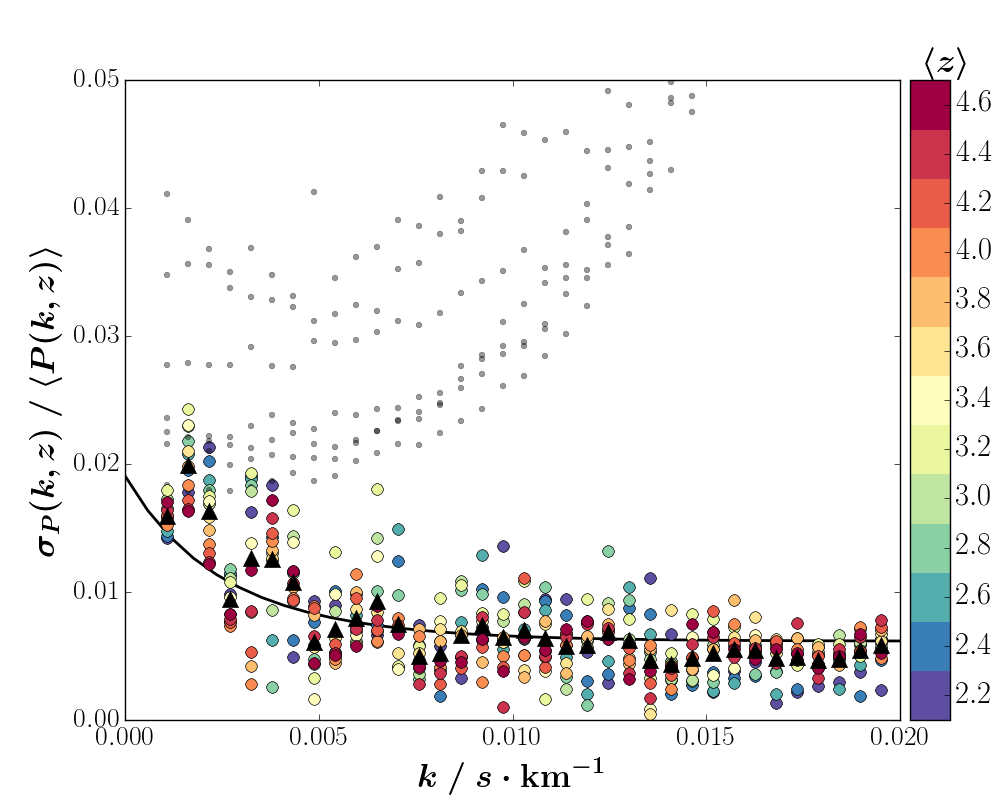
\includegraphics[width=0.8\columnwidth]{Sample_Var.png}
\caption{Sampling uncertainty as function of $k$ and $z$ (color code) for the power spectrum averaged over the 5 different seeds. The average accross the 13 redshift bins at each $k$ is given by the black triangles, and the black curve is the best fit of the form given in Eq.~\ref{eq:variance_fit}. The small grey dots are the BOSS data statistical uncertainty for comparison.}
\label{fig:sampling_variance}
\end{center}
\end{figure}


%%%%%%%%%%%%%%%%%%%%%%%%%%%%%%
\subsection{The \texttt{Gadget} Code}
%%%%%%%%%%%%%%%%%%%%%%%%%%%%%%

\subsubsection{Smoothed Particle Hydrodynamics: Baryons}
\label{sec:sph}

To describe the evolution of baryons in our simulations, we require the equations of motion which are grouped in the Vlasov-Poisson system in Eq.~\ref{sys:sph_eq}. For a gas particle of mass density $\rho$, internal energy per unit mass $\varepsilon$, exerting pressure $\mathcal{P}$, in motion at peculiar velocity $\vec{v}$ in a gravitational field $\phi$ in an expanding volume, \\

\begin{equation}
\label{sys:sph_eq}
\left\{
\begin{array}{l}
\partial_t ~\rho + \vec{\nabla} \cdot \left( \rho \vec{v} \right) = 0 \\
\\
\partial_t ~\vec{v} + \left( \vec{v} \cdot \vec{\nabla} \right) \cdot \vec{v} + \vec{\nabla} \left( \mathcal{P}/\rho + \phi \right) = \vec{0} \\
\\
\partial_t ~\varepsilon + \left( \vec{v} \cdot \vec{\nabla} \right) \left( \varepsilon + \mathcal{P}/\rho + \phi \right) = 0\\
\\
\nabla^2 \phi = 4 \pi G~ a^2 ~\delta
\end{array}
\right.
\end{equation} \\

The first (continuity) equation expresses the conservation of mass. The second and third Euler equations stem from the conservation of momentum and energy respectively and can be obtained from simplifying the Einstein equations. The last equation is the Poisson equation, where $\rho = \bar{\rho} (1+\delta)$ and $a$ is the scale factor. In the context of cosmology, gases obey a \emph{polytropic} equation of state of the form

\begin{equation}
\mathcal{P} \propto \rho^\gamma
\end{equation} 

with $\gamma$ the adiabatic index, or heat capacity ratio ($5/3$ for a monoatomic gas, $7/5$ for a diatomic gas). Discretizing these equations are a computational challenge. A popular method to solve them in the Lagrangian framework is Smoothed Particle Hydrodynamics (SPH). The general idea is to approximate the density profile around a particle of gas by the Gingold Monaghan Lucy estimator \citep{Gingold1977, Lucy1977}:

\begin{equation}
\label{eq:SPH_estimator}
\rho(\vec{r}) = \sum_{i=1}^{N^3} m_i~W(x_i, \ell)
\end{equation} 

where $\ell$ is a smoothing length scale, $x_i = \vert \vec{r} - \vec{r}_i \vert / \ell$ the reduced distance to particle $i$ and $W$ a weighing kernel. The typical choice for the smoothing scale, which governs the decrease of the $W$ function with distance, is the radius of the sphere within which the mass remains constant \citep{Springel2002}. The smoothing kernel must be positive, symmetric, unitary\footnote{its integral over space must be $1$} by virtue of the conservation of mass ($\int d^3\vec{r}~\rho(\vec{r}) = \sum_i m_i$), have a flat core ($\left. dW/dx \right\vert_{x=0} = 0$) so that the density isn't strongly altered by a small displacement of a neighboring particle, and decrease smoothly. The issue with the most natural choice for $W$, \textit{i.e.} the Gaussian kernel \\
\begin{equation}
\label{eq:gausskernel}
\displaystyle W_{\mathrm{gauss}}(x_i, \ell) = \cfrac{e^{- x_i^2}}{\ell^3 \pi \sqrt{\pi}}
\end{equation} \\ is that its infinite range makes it too computationally expensive. It is far more advantageous to neglect the interaction between two particles a few smoothing length scales away from one another. Nowadays, a popular choice for a smoothing kernel is the cubic spline \citep{Monaghan1985}, illustrated in Fig.~\ref{fig:spline}: \\
\begin{equation}
\label{eq:cubekernel}
W_{\mathrm{cube}}(x_i, \ell) = \frac{1}{\pi} \times
\begin{cases}
1 + x_i^2 (-\cfrac{3}{2} + \cfrac{3}{4} x_i) & \text{for}~0 \leqslant x_i < 1 \\
\cfrac{1}{4} (2-x_i)^3 & \text{for}~1 \leqslant  x_i < 2\\
0 & \text{for}~x_i \geqslant 2
\end{cases}
\end{equation} \\

\begin{figure}
\centering
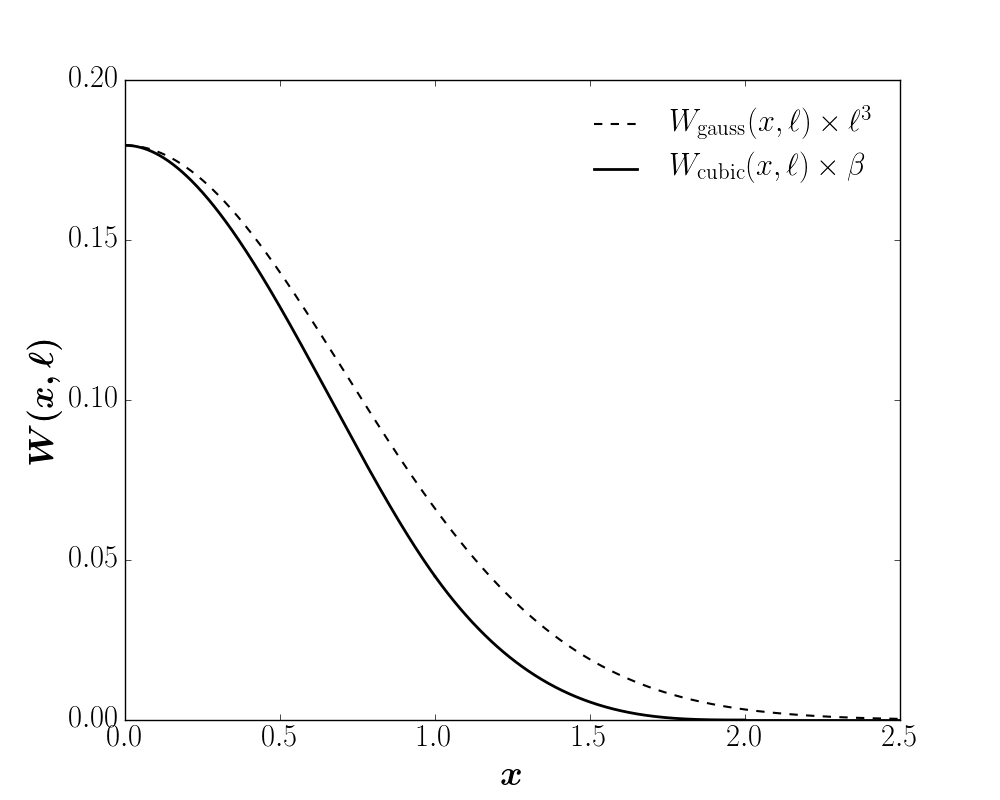
\includegraphics[width=0.75\textwidth]{Simu/CubicSpline.png}
\caption{Gaussian and cubic spline kernels defined in Eq.~\ref{eq:gausskernel} and \ref{eq:cubekernel}, as functions of the distance to a particle: $x = \vert \vec{r} - \vec{r}_i \vert / \ell$ reduced by the smoothing length. The Gaussian kernel is multiplied by $\ell^3$, while the cubic spline is normalized such that $\ell^3 \times W_{\mathrm{gauss}} (0) = W_{\mathrm{cubic}} (0)$ for illustrative purposes.}
\label{fig:spline}
\end{figure}

The details of the calculations can
be found in \cite{Price2012}. More complete reviews and discussions of SPH can be found in \cite{Monaghan1992},
\cite{Monaghan2005}, \cite{Rosswog2009}, \cite{Springel2010} and  \cite{Price2011}. Grid based codes like \texttt{RAMSES} \citep{Teyssier2002} or \texttt{ENZO} \citep{Bryan2013} which are using adaptive mesh
refinement (AMR), solve the hydrodynamical equations using the Godunov scheme \citep{Godunov1959} extension in which data are no longer approximated by piecewise constant functions but rather piecewise linear functions \citep{VanLeer1979} or piecewise parabolic functions \citep{Colella1984, Woodward1984}.

\subsubsection{N-body: Dark Matter and Neutrinos}
\label{sec:nbody}

When neutrinos become non-relativitic, \textit{i.e.} when $T \sim m_\nu^{\mathrm{eff}}$, their kinetic energy becomes comparable and increasingly subsidiary to their rest mass and one can use a point particle approximation to fully describe their motion. Such is the case for any dark matter particle, hot warm or cold, once they've gone non-relativistic.  The main difference between dark matter particles including neutrinos with baryons is that they are poorly or non-interacting. The SPH treatment described above does not apply to these particles. In the simulations I operate, I explicitely distinguish active sub-eV neutrinos from cold dark matter particles for the sole reason that the velocity distribution of the former cannot be neglected. The thermal velocities of neutrinos is taken into account from their mass, which fully determines their distribution given their energy density $\Omega_\nu$ since they are assumed to be thermalized. In simulations where $\Sigma m_\nu$ is explicitely non-zero, the simulation comoving volume contains an additional $N^3$ neutrinos for a total of $3\times N^3$ particles. For simulations investigating non-cold dark matter cosmologies, the WDM particle is non-relativistic in the Matter Dominated Era and at $z=30$ it is reasonable to adopt the point particle approximation as well. For pure WDM and cool DM, the thermal velocities are negligeble (see Tab.~\ref{tab:vth}) and it is un-necessary to include the additional neutrino population in \texttt{2LPTic} and \texttt{Gadget}. For C+WDM, the warm component's velocity with respect to the cold is negligeable as well and so the dark matter component is treated as a mono-fluid whose transfer function is given by Fig.~\ref{fig:pk_cwdm}, without the need of including the additional neutrino component in the simulations. Only the C+HDM simulations require involving the neutrino component since their thermal velocities not only aren't negligeable but are of the order several $10^{3-4}~\mathrm{km/s}$ for eV scale neutrinos, as is relayed in Tab./~\ref{tab:vth_chdm}. In that case \texttt{2LPTic} requires not only the transfer function of the massive neutrinos but generates the velocity distribution as well, making the total number of particles in the simulation $3 \times N^3$ instead of $2 \times N^3$ for the other 3 projects (C+WDM, WDM, cool DM) as well as the benchmark CDM.\\

\begin{table}
	\begin{center}
	\begin{small}
		\begin{tabular}{cc}
			$\pmb{\sum m_\nu / \mathrm{eV}}$ & $\pmb{\langle v_{\mathrm{th}}^\nu \rangle (z=30)}$\\[2pt]
			\hline \\[-10pt]
			\\[-10pt]
			$0.8$ & $6.08 \times 10^3~\mathrm{km}/s$ \\[2pt]
			$0.4$ & $12.17 \times 10^3~\mathrm{km}/s$ \\[2pt]
			$0.2$ & $24.34 \times 10^3~\mathrm{km}/s$ \\[2pt]
			$0.1$ & $48.67 \times 10^3~\mathrm{km}/s$ \\[2pt]
			\hline \\[-10pt]
		\end{tabular}
	\end{small}
	\end{center}
	\caption{thermal velocities at $z=30$ for left-handed neutrinos incorporated in our C+HDM simulations}
	\label{tab:vth_chdm}
\end{table}


Solving the N-body problem comes down to numerically solving the Poisson equation in system \ref{sys:sph_eq}. Doing so for each and every particle would be too costly, despite being exact. The \texttt{Gadget} code uses a tree-PM algorithm, which stands for hierarchical tree and particle mesh. The tree is used to compute the interactions between particles on short scales after dividing the overall distribution of particles into a hierarchy of groups. In each group, the gravitational interaction is computed on all particles in that group. At the next level of hierarchy, the gravitational interaction between those distant groups is computed on their barycenters; iteratively so until the code has reached the single node at the tree trunk. The advantage of the hierarchical tree is that it is relatively accurate compared to other methods, and the level of precision can be explicitely specified by the user. The particle mesh method on the other hand is performed on large scales. It maps the particles on a uniform grid and solves for the gravitational potential via the Poisson equation in Fourier space before differentiating the potential at the particle's positions. The advantage of that method is its speed. \texttt{Gadget} uses both methods to solve the N-body problem for $N^3$ dark matter particles and $N^3$ neutrino particles when specified, in addition to solving the full set of hydrodynamics equations in system \ref{sys:sph_eq} using SPH for $N^3$ baryon particles. The concept of "particle" in this context is a bunch of particles occupying the same phase-space volume, of several solar masses depending on the resolution.

\subsubsection{Code Description}
\label{sec:gadget_description}
\texttt{GADGET-3} (GAlaxies with Dark matter and Gas intEracT) is a massively parallel tree-SPH code written in ANSI C for cosmological simulations, originally developed by Volker Springel and collaborators \citep{Springel2001,Springel2005}. It uses the standardized message passing interface (\texttt{MPI}) along with several open-source libraries (\texttt{GSL}\footnote{\url{http://www.gnu.org/software/gsl/}}, \texttt{FFTW}\footnote{\url{http://www.fftw.org/}}). Gravitational interactions are computed via a hierarchical multipole expansion using the standard $N$-body method, and gas-dynamics are followed with smoothed particle
hydrodynamics (SPH); collisionless dark matter and gas are both represented by particles. 

Since its original version (\texttt{Gadget-1}), the code underwent a series of improvements and 
optimizations over several years (\texttt{Gadget-2} and \texttt{3}), to maximize the work-load balance and the efficiency in memory consumption and communication bandwidth. In what follows, we briefly describe the key features of the code. \\

\texttt{Gadget-3} follows a collisionless fluid with the standard $N$-body method, and an ideal gas with smoothed particle hydrodynamics (SPH). The code solves simultaneously for the dynamics of the collisionless component and of the ideal gas, both subject to and coupled by gravity in an expanding background space. The $N$-body implementation only differs from other cosmological codes by the accuracy of the gravitational field computation. A number of further physical processes have also been implemented in \texttt{Gadget-3}, from radiative cooling/heating physics to non-standard dark matter dynamics, star formation and feedback. Fig.~\ref{fig:slices}, presents the evolution of a filament with redshift and in Fig.~\ref{fig:visu_seed} I show the image of a snapshot rendered with \texttt{Splotch}\footnote{\url{http://www.mpa-garching.mpg.de/~kdolag/Splotch}}. Such renderings can be used for both visual inspection before
quantitative analysis (which was useful several times) as well as for public outreach and education. I've made several $\sim 30$ second motion picture sequences which I've presented at the Paris \textit{Palais de la D\'ecouverte}\footnote{\url{http://www.palais-decouverte.fr/fr/accueil/}} for outreach and presentation of our computational endeavor at the cosmological group in Saclay, as well as a $\sim 2$ minute motion picture sequence in 3D as part of the public outreach movie ``\textit{L'Univers Recalcul\'e}''.\\

Several optimization strategies have been added in \texttt{Gadget-3}. These include a Peano-Hilbert space decomposition, a massively parallel version of the Fast Fourier Transform library,  the possibility of splitting the simulation data across several files (to facilitate and speed-up the input/output process), and the fact that the code can be run on an arbitrary number of processors. In its current version, \texttt{Gadget-3} is highly efficient in memory consumption (it allocates up to $80$ bytes per particle) and communication bandwidth, is versatile and flexible, accurate and fast. Another important aspect  is the scalability of the code, i.e. its
performance when the number of processors is increased, which has currently been tested up to $16,000$ cores.\\

\begin{figure}
\centering
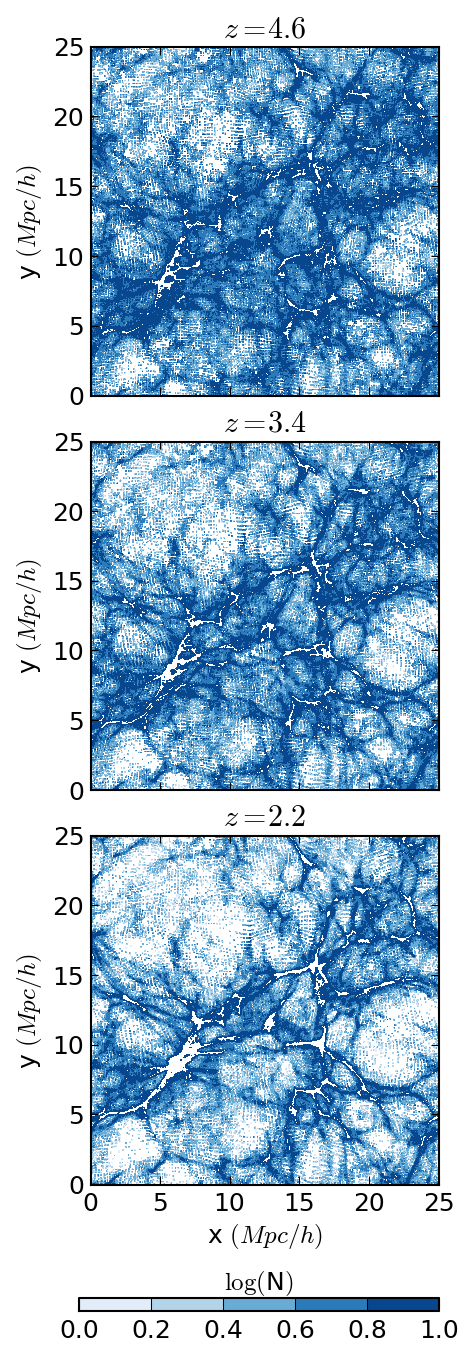
\includegraphics[height=0.87\textheight]{Simu/gas_slice.png}
\hfill
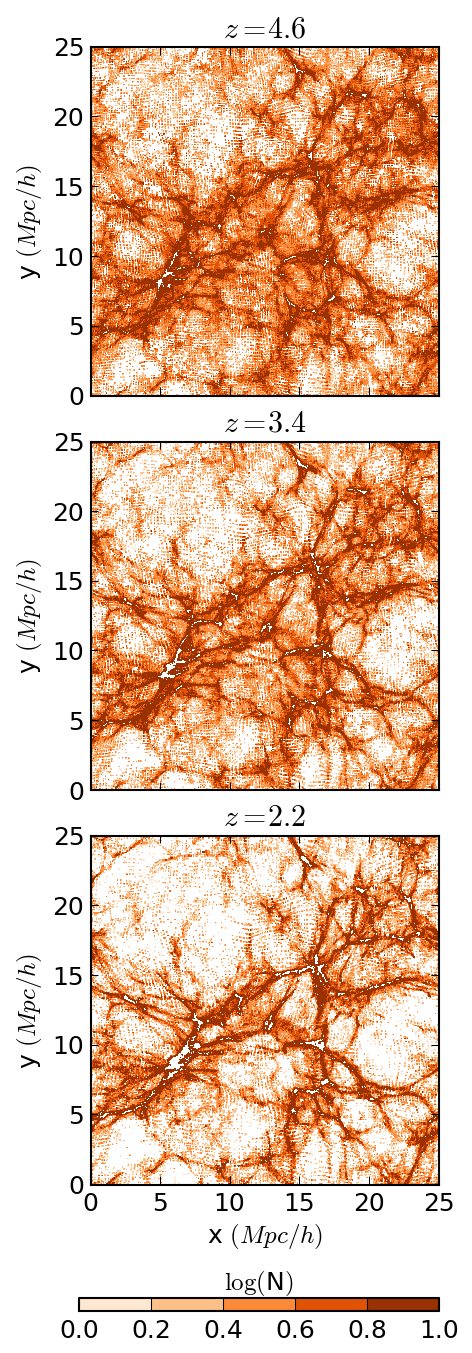
\includegraphics[height=0.87\textheight]{Simu/dm_slice.png}
\caption{Slice of baryon and dark matter snapshots ($2.5~h^{-1}\mathrm{Mpc}$ depth), at three different redshifts, extracted from a simulation with $192^3$ particles per type in a 
$25~(h^{-1}\mathrm{Mpc})^3$ box. As expected, there are very few
differences between the distributions for the two types of particles. Color represents particle number density. Out-of-scale densities (whether underflow or overflow) are white.}
\label{fig:slices}
\end{figure}

We started all our simulations at $z_{\mathrm{ic}}=30$ with initial conditions based on second-order Lagrangian perturbation theory\citep{Crocce2006}, and adopted the same gravitational softening for the different species considered (\textit{i.e.} gas, dark matter, stars), which however varies with the length of the box and the size of the mesh chosen. Specifically, we set the gravitational softening length to $0.8~h^{-1}\mathrm{kpc}$ for the simulation having $25~h^{-1}\mathrm{Mpc}$ boxsize and $N=768$, while the softening is $3.25~h^{-1}\mathrm{kpc}$ for the other two runs, \textit{i.e.} the $25~h^{-1}\mathrm{Mpc}$ boxsize and $N=192$ and the $100~h^{-1}\mathrm{Mpc}$ boxsize and $N=768$.  We used the `QUICKLYA' routine in \texttt{Gadget-3} to simulate the Lyman-$\alpha$ forest, assuming the gas of  primordial composition with a helium mass fraction of $Y=0.24$. We neglect metals and the evolution of elementary  abundances, as well as feedback processes and galactic winds. Along the lines of \cite{Viel2010}, we adopted a simplified criterion for star formation: all gas particles whose overdensity with respect to the mean is above 1000 and whose temperature is less than $10^5~\mathrm{K}$ are turned into star particles immediately. 


\clearpage